\documentclass[12pt,a4paper]{book}
\usepackage[utf8]{inputenc}	
\usepackage[spanish]{babel}
\usepackage{amsmath}
\usepackage{amsfonts}
\usepackage{amssymb}
\usepackage{graphicx}
\usepackage{fourier}
\usepackage[left=2cm,right=2cm,top=2cm,bottom=2cm]{geometry}
\usepackage{hyperref} %Paquete para agregar hipervínculos

\usepackage{subfigure} % subFiguras
\usepackage{float} %fijar Figuras
\usepackage{listings} %este paquete esta agregado para que se pueda agregar lineas de código de programa (en este caso FORTRAN) a nuestro documento



\spanishdecimal{.}

%\usepackage{cancel} %cancelar términos
%\usepackage[backend=biber]{biblatex}
%\addbibresource{biblio.bib}

\providecommand{\abs}[1]{\lvert#1\rvert} %agregación para el valor absoluto
\usepackage{xcolor}
\usepackage{graphicx}
%\usepackage{subfigure} % subFiguras
\lstset{language=Fortran, %nuestro lenguaje fortran por su pollo
backgroundcolor=\color{white}, %color de fondo blanco para eso es que ocupe el paquete color
basicstyle=\footnotesize, % Fija el tamaño del tipo de letra utilizado para el código
breakatwhitespace=false,% Activarlo para que los saltos automáticos solo se apliquen en los espacios en blanco
breaklines=true,
commentstyle=\color{blue}, %color de los comentarios del código
keepspaces=true, 
rulecolor=\color{black}, % Si no se activa, el color del marco puede cambiar en los saltos de línea entre textos que sea de otro color
keywordstyle=\color{red},% estilo de las palabras clave
stringstyle=\color{yellow},% Estilo de las cadenas de texto
stringstyle=\color{orange}, 
}
\lstset{numbers=left, numberstyle=\tiny, stepnumber=1, numbersep=-2pt}

\author{Julio César Sosa Mondragón}

\begin{document}

\begin{minipage}{.3\textwidth}
  
  \flushleft
  \center{
\includegraphics[scale=.09]{unam.pdf}}

  \vspace{20pt}

  \center{
    \rule{.5pt}{.6\textheight}
    \hspace{7pt}
    \rule{2pt}{.6\textheight}
    \hspace{7pt}
    \rule{.5pt}{.6\textheight}
         } \\

\center{
\includegraphics[scale=.22]{ciencias.pdf}}
\end{minipage}
\begin{minipage}{.7\textwidth}

\flushright

\center{

  \center{
    \LARGE{U}\large{NIVERSIDAD} \LARGE{N}\large{ACIONAL} 
    \LARGE{A}\large{UTÓNOMA} \\[10pt]
    \large{DE} 
    \LARGE{M}\large{ÉXICO} 
  } \\
  \rule{\textwidth}{2pt}
  \\
  \hrulefill\\[1cm]
  
  \LARGE{F}\large{ACULTAD DE } \LARGE{C}\large{IENCIAS}\\[2cm]

  \large{
Simulaciones numéricas hidrodinámicas relativistas de Destellos de Rayos Gamma cortos lanzados desde un objeto compacto en varios tipos de medios ambientes. }\\[2cm]

  \huge{
T \hspace{1cm} E \hspace{1cm} S \hspace{1cm} I \hspace{1cm} S  }\\[1cm]

  \large{QUE PARA OBTENER EL TÍTULO DE:}\\[1cm]

  \large{
Físico  }\\[1cm]

  \large{PRESENTA:}\\[1cm]

  \large{
Julio César Sosa Mondragón  }\\[1cm]

  \large{
TUTOR  }\\[1cm]

  \large{
Dr. Diego López Cámara Ramírez}
}

\end{minipage}
\thispagestyle{empty} % para que no se numere esta pagina


\pagenumbering{Roman} % para comenzar la numeracion de paginas en numeros romanos
\tableofcontents % indice de contenidos

%
%%\cleardoublepage
%%\addcontentsline{toc}{chapter}{Lista de Figuras} % para que aparezca en el indice de contenidos
%%\listoffigures % indice de Figuras
%
%%\cleardoublepage
%%\addcontentsline{toc}{chapter}{Lista de tablas} % para que aparezca en el indice de contenidos
%%\listoftables % indice de tablas
%
%%%%%%%%%%%%%% DEDICATORIA %%%%%%%%%%%%%%%%%%%%%%%%%%%%%%%%%%%
\chapter*{Dedicatoria}

\addcontentsline{toc}{chapter}{Dedicatoria}
%
\begin{flushright}
\textit{Dedicado a \\
mi familia}
\end{flushright}

%%%%%%%%%%%%%%%%%%%%%%%%%%%%%%%%%%%%%%%%%%%%%%%%%%%%%%%%%%%%%%%%%%
%
\chapter*{Agradecimientos} % si no queremos que añada la palabra "Capitulo"
\addcontentsline{toc}{chapter}{Agradecimientos} % si queremos que aparezca en el índice
\markboth{AGRADECIMIENTOS}{AGRADECIMIENTOS} % encabezado
 
¡Muchas gracias a todos!
%%%%%%%%%%%%%%%%%%%%%%%%%%%%%%%%%%%%%%%%%%%%%%%%%%%%%%%%%%%%%%%%%%%%%

\chapter*{Resumen} % si no queremos que añada la palabra "Capitulo"
\addcontentsline{toc}{chapter}{Resumen} % si queremos que aparezca en el índice

\markboth{RESUMEN}{RESUMEN} % encabezado
%
Una bonita historia
%
%%%%%%%%%%%%%%%  CAPITULOS %%%%%%%%%%%%%%%%%%%%%%%%%%%%%%%%%%55
%
%

\chapter{Introducción}

\pagenumbering{arabic} % para empezar la numeración con números
%Érase una vez...

Los destellos de rayos gamma (GRB por su acrónimo en inglés) son eyecciones de rayos gamma del orden de Mev, son cortos, intensos y no repetitivos.
Estos consisten en la emisión de energías altas como los rayos $\gamma$ y los rayos X, asi como energías bajas como el óptico, el radio, entre otros \cite{PGRB-piran}. %Piran2005
Fueron descubiertos por los satélites \emph{Vela}\footnote{\url{https://heasarc.gsfc.nasa.gov/docs/heasarc/missions/vela5a.html}} a finales de la decada de los 60's, gracias a los datos recabados por el experimento BATSE\footnote{\url{https://gammaray.msfc.nasa.gov/batse/}} se logró identificar 2 grupos principales de GRBs, los cortos y los largos, en los cuales este último tiene una duracion mayor a los 2 s \cite{Berger:2013jza}.

\begin{figure} 
%fuente de la imagen: https://imagine.gsfc.nasa.gov/science/objects/bursts1.html
  \centering
    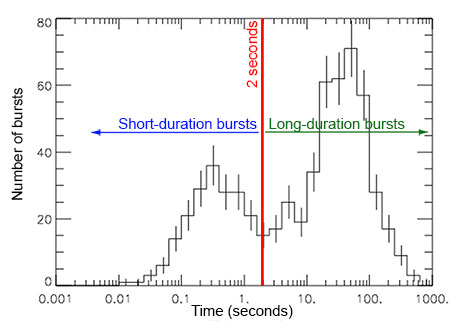
\includegraphics[width=0.5\textwidth]{Figuras/burst_durations_labelled.jpg}
  \caption{Gráfico que muestra la diferencia de tiempo que existe entre GRBs cortos y GRBs largos. Se pueden apreciar 2 picos que marcan la diferencia de duracion entre los GRBs}
  \label{fig:Batse_duration_GRBs}
\end{figure}

El objetivo principal del estudio de los GRBs es analizar las propiedades de los estallidos de los rayos gamma, así como sus progenitores y determinar las propiedades básicas de estos, la fusión de objetos compactos es el modelo progenitor más atractivo.
Las categorías de los GRBs largos y cortos son aproximadamente 75\% y 25\% de la población \cite{GRB:PPP}. %Gamma Ray Burst Progress, problems and prospects Zhang, meszaros
La interacción de flujos de salida relativistas con el medio ambiente que lo rodea produce emisión sincrotrónica que va desde la banda de las ondas de radio a los rayos X, los GRBs son uno de los eventos que más libera energía en el universo \cite{Berger:2013jza}, la energía liberada es del orden de $10^{52}$ ergs.

Aunque hay mucha información acerca de los GRBs largos, los cortos son aún un estudio nuevo en el área de astrofísica de altas energías ya que debido a su corta duración son difíciles de estudiar. 
\section{Características de los GRBs}
Muchas de las características de los GRBS ya sean estos largos o cortos, son la duración media que tienen, mientras que en los GRBs largos tienen un promedio de duración de 100 s \cite{PGRB-piran}, los GRBs cortos duran menos de 2 segundos. Los estallidos de Rayos gamma se encuentran a miles de años luz de nuestra galaxia por lo que se puede decir que tienen un orígen cosmologico, mientras los GRBs largos se originan en los centros de las galaxias, los cortos lo hacen lejos de la galaxia donde se originaron y por consecuencia, estos tienen una densidad de ambiente muy bajo. El estudio de los SGRB ha sido muy difícil debido al tiempo de duración que conllevan estos eventos y a la dificultad de asociarlo con galaxias anfitrionas. 

%Las partes principales de los GRBs son la emisión propmt y  afterglow. %Piran2005

\begin{figure} %fuente de la imagen:https://astrobites.org/2017/11/13/grb-afterglows-coming-out-of-a-cocoon/
  \centering
    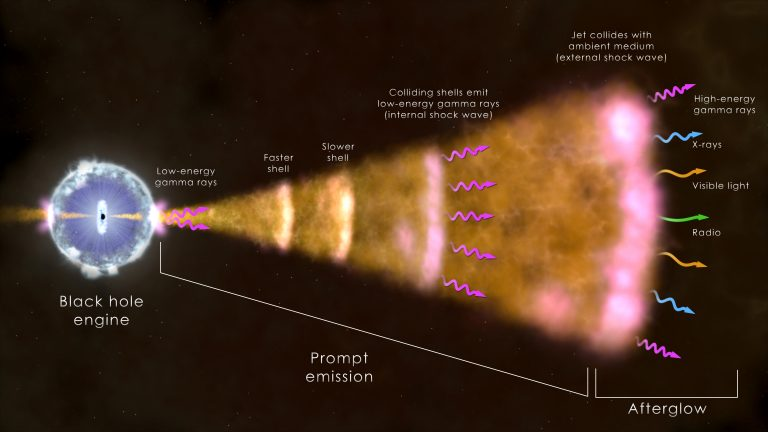
\includegraphics[width=0.5\textwidth]{Figuras/Gamma-ray_burst_by_a_blackhole-768x432.jpg}
  \caption{Diferentes partes de un GRB en general, mostrando las partes más características como el afterflow y la emisión prompt}
  \label{fig:Partes de GRBs}
\end{figure}


\subsection{Emisión pronta} %Azzam
La emisión pronta es definido como el periodo de tiempo donde el detector de rayos $\gamma$ 
detecta una señal sobre el fondo. Estas consisten en fotones de alta energía, no tiene espectro térmico \cite{GRB:CAP}. El espectro térmico es producido por un gas en equilibio térmico. Además, tiene bastantes carterísticas observacionales.

El flujo de energía varía dentro de cientos de Kev. La emisión de las curvas de luz son notoriamente irregulares sobre escalas de tiempo muy pequeñas \cite{SGRBr-Avanzo}(ver Figura \ref{lightcurve}). %Short gamma-ray bursts: A review; P. D’Avanzo
En los GRBs cortos, su espectro de emisión, se ha encontrado más duro que en los GRBs largos, esto debido a que es una combinación de componentes espectrales duros de baja energía. Una característica de principal es la duración de esta emisión, esta llega a ser del orden $\geq \, 10^{-2} $ s a $10^{3}$ s \cite{GRB:PPP}. Los valores promedio de dichas emisiones son $t \sim 20 $ s para GRBs largos y $t \sim 0.2 $ s para los cortos \cite{GRB:PPP}. %Gamma Ray Burst Progress, problems and prospects Zhang, meszaros

\begin{figure}
\centering %Fuente Zhang
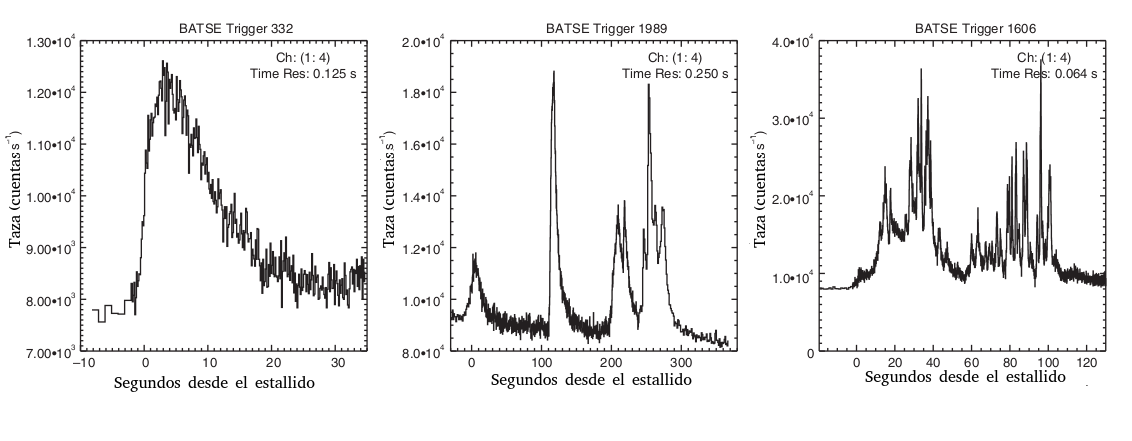
\includegraphics[width=1.0\textwidth]{Figuras/lightcurve_different}
\caption{\label{lightcurve} Diferentes curvas de luz captadas por el detector Batse detectadas en la emisión pronta de los GRBs. Las curvas de luz difieren bastantes unas de otras, mientras que BATSE 332 es un decaimiento exponencial , BATSE Trigger 1989  tiene 2 picos de intensidad. }
\end{figure}
\subsection{Emisión tardía}
La emisión tardía,conocida tambien como \emph{afterglow},  es después de la emisión prompt en el cual se pueden detectar otras longitudes de onda como el óptico, radio y los rayos X \cite{Berger:2013jza, PGRB-piran, SGRBr-Avanzo}. %\ref{fig:Partes de GRBs}.
La propiedad de "multiples longitudes de onda", hace una propiedad única de la emisión tardía. Estos cubren un amplio rango de frecuencias, desde las ondas de radio hasta los Tev. El espectro de banda ancha es descrito como una ley de potencias inversa, ya que la fuerza del choque se reduce a medida que la onda expansiva va desacelerando. Con lo que se espera que todas las longitudes de onda de las curvas de luz decaigan como ley de potencias. Entonces la densidad de flujo es proporcional a:

\begin{equation}
F_{\nu}(t,\nu) \propto t^{-\alpha} \nu^{\beta}
\end{equation}

Donde $\alpha$ y $\beta$ son reales positivos.


En Mayo y Julio del 2005 datos de eyecciones recopiladas por el satélite \emph{swift} al seguir al seguir al GRB 050509B, descubrieron las primeras fases tardías de los GRBs cortos, tiempo después el satélite HETE-2 junto con el observatorio \emph{chandra} de rayos X siguieron al satélite 050709 el cual localizo la fase tardía en rayos X y despues en la banda óptica, con estos datos recabados de la fase tardía se pudo llegar a que los GRBs cortos tienen una escala de densidad y una energía mas baja que los GRBs largos, tambien se llego a la conclusión de que los GRBs cortos tienen orígenes cosmologicos \cite{Berger:2013jza} y que las estrellas masivas no son sus progenitores como en el caso de GRBs cortos.
 
\subsection{Energía y luminosidad}
Los GRBs largos tienen una luminosidad isotrópica $L_{iso} \sim 10^{49}-10^{54} \, \mathrm{ergs} \cdot \mathrm{s}^{-1}$. También  hay GRBs largos con una luminosidad baja, sus valores rondan acerca de $L_{iso} \sim 5 \times 10^{46}-10^{49} \, \mathrm{ergs} \cdot \mathrm{s}^{-1}$, pero estos son solo una pequeña fracción de los GRBs largos observados. Los GRBs cortos tiene generalmente una luminosidad de $L_{iso} \sim 10^{49} \, \mathrm{ergs} \cdot \mathrm{s}^{-1}$.

La distribución de energías es amplia para los GRBs, estos cubren valores $E_{iso} \sim 10^{49}-10^{55}$ ergs para los largos y para los cortos $E_{iso} \sim 3.3 \times 10^{46}-10^{53}$ ergs \cite{Zhang:PGRB}. %the physics of gamma ray burst

%
\section{Características de los GRBs cortos}
Los GRBS cortos, aunque tiene muchas carcteristicas en común con los GRBs largos, también tienen sus propias peculariedades que lo hacen diferente del otro.

\subsection{Progenitores} %ghrels2009
Los GRBs cortos por lo general se localizan en medios de baja formación estelar por lo que no se espera poder encontrarlos ambientes estelares jovenes además de que, conllevan una carencia para poder asociarlos con SNs. El modelo más aceptado en la literatura de los progenitores de los GRBs cortos son la fusión de objetos compactos binarios. Estos pueden comprender a dos estrellas de neutrones (NS-NS), una estrella de neutrones y un agujero negro (NS-BH) o dos agujeros negros (BH-BH) \cite{GRB-SE}. La fusión se logra a cabo debido a la pérdida de momento angular y energía debido a las ondas gravitacionales. La interacción de este fenómeno lleva a la extracción de energía por procesos magnetohidrodinámicos (MHD), los cuales impulsan un flujo relativista colimado. 

Las patadas natales pueden ser las causantes de las distancias en las que estos nacen y los sitios de explosión de estos sistemas \cite{Berger:2013jza}, la probabilidad para una galaxia de brillo $m$  a ser localizada a una separación $\delta R$ de la posición de un SGRB está dada por 

\begin{equation}
P_{cc} = 1 - \exp ^{- \pi (\delta R)^{2} \sum(\leq m)}
\end{equation}
Donde $\sum(\leq m) = 1.3\cdot 10^{0.33(m-24)-2.44} \mathrm{arcsec} ^{-2}$ son el número de cuentas de la galaxia. Los SGRBs sin galaxias anfitrionas se exhiben cerca galaxias de campo con una baja probabilidad de coincidencia, generalmente las distancias medias de separación del SGRB con su galaxia anfitriona es de $ \frac{\delta R}{r_e} \approx 1.5$ donde $r_e$ es el radio estelar. 

\subsection{Propiedades de las explosiones de los SGRB}

Los parámetros claves de interés de la emisión pronta y tardia \cite{Berger:2013jza}
\begin{itemize}
\item $E_{\gamma}$: Energía de rayos $\gamma$.
\item $E_k$: Energía cinética de la onda de choque de la emisión tardía.
\item $\theta_j$: El ángulo de apertura del jet.
\item $n$: Densidad del medio ambiente.
\end{itemize}

La emisión del sincrotrón de la emisión tardía incluye dos parámetros libres que tienen relación con la física del choque relativista:
\begin{itemize}
\item $\epsilon_{B}$: Fracción de energía del post-choque de los campos magnéticos.
\item $\epsilon_e$: Radiación relativista de los electrones. 
\end{itemize}



El flujo relativista interactuando con el medio circundante es el espectro de emisión sincrotónico. Esta se caracteríza por 3 frecuencias de corte:
\begin{itemize}
\item $\nu_a$: Auto absorción
\item $\nu_m$: Factor mínimo de Lorentz
\item $\nu_c$: enfriamiento sincrotrónico
\end{itemize}

Tomando en cuenta los valores de estos parámetros y la pendiente del espectro para $\nu < \nu_m$ se pueden llegar a encontrar los siguientes valores $E_{k, \, \mathrm{iso}}$, $n$, $\epsilon_{B}$ y $\epsilon_e$. La evolución temporal del espectro también se puede usar para encontrar el ángulo de apertura del jet $\theta_j$. La relacción que existe entre el ángulo de apertura $\theta_j$ y el tiempo $(t_j)$ al cual ocurre el jet break  está dado por la siguiente fórmula.

%La mayoría de estas frecuencias se encuentran entre 1 $\thicksim$ 10 GHz por lo cual ha sido difícil de detectarlas. La colimación del jet también influye en la taza de los SGRBs y proporciona una restricción adicional al modelo progenitor, la firmatura de la colimación de los destellos de los SGRBs son los llamados "Jet Break" que ocurren al tiempo $t_j$ cuando $\Gamma_j(t_j) = 1/ \theta_j$, esto lidera al cambio de emisión del espectro sincrotrónico
%
%\begin{equation}
%F_\nu \propto t^{-1} \longrightarrow F_\nu \propto t^{-p}
%\end{equation}
%
%La relación entre el "jet break" y el ángulo de apertura esta dado por:
%
\begin{equation}
\theta_j = 0.13 \left( \frac{t_{j,d}}{1+z} \right)^{3/8}
\left(\frac{n_0}{E_{52}} \right)^{1/8}
\end{equation}
%
%\section{GRB del 17 de agosto del 2017}
%

\begin{figure}
\centering
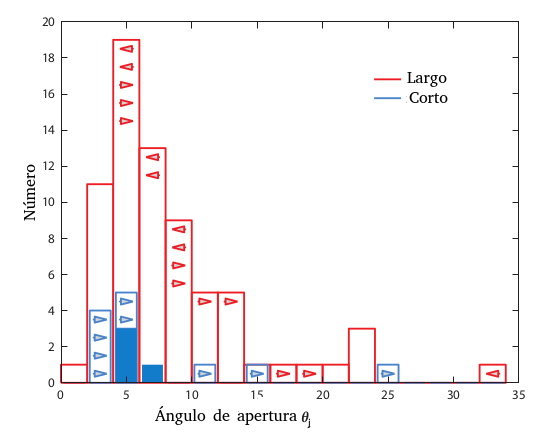
\includegraphics[scale=0.7]{./Figuras/Distribucion_angulo_apertura}
\caption{La Figura muestra la distribución de los ángulos de apertura para los GRBs largos (rojos) y los GRBs cortos (azules). Las flechas muestran el límite superior e inferior de los ángulos. }
\end{figure}

\chapter{Teoría}

Los GRBs, ya sean largos o cortos, que se originan en el medio interestelar, se pueden describir como un fluido sin viscosidad y estos pueden ser descritos bajo
las ecuaciones de la hidrodinámica.
Para describir un sistema de partículas como un fluido bajo ciertas condiciones uno debe de conocer que el camino libre medio debe de ser mucho mas pequeño que la escala de longitud de las fluctuaciones de las variables macroscópicas.

\begin{equation}
\lambda_{mfp} \ll L
\end{equation}

El tiempo entre las colisiones debe de ser pequeña comparada con la escala del tiempo de los cambios en el fluido
\begin{equation}
t_{c} \ll t_f
\end{equation}
La distancia media entre las partículas tiene que ser mas pequeña que la longitud de escala de las variables macroscópicas

\begin{equation}
l = n^{-1/3} \ll L
\end{equation}

\section{Ecuaciones de la hidrodinámica}


Considerando una serie de elementos de volumen fijos, las ecuaciones que describen el movimiento de un fluido sin considerar efectos viscosos son:

La conservación de masa
\begin{equation} \label{conservación_masa_hidrodinamica}
\dfrac{\partial \rho }{\partial t} + \nabla \cdot \left( \rho \mathbf{u} \right)
\end{equation}

El momento
\begin{equation}  \label{conservacion_momento_hidrodinamica}
\dfrac{\partial \left( \rho \mathbf{u} \right) }{\partial t}+ \nabla \cdot \left( \rho \mathbf{u u} \right) + \nabla p = \mathbf{f_{ext}}
\end{equation}

Ecuación de la energía

\begin{equation} \label{conservacion_energia_hidrodinamica}
\dfrac{\partial E }{\partial t} + \nabla \cdot \left[ \mathbf{u} \left( e+p \right) \right] =G-L+\mathbf{f_{ext} \cdot \mathbf{u}}
\end{equation}

Ecuación de estado
\begin{equation}
e=\frac{1}{2} \rho \mathbf{u}^{2} + \frac{p}{\Gamma - 1}
\end{equation}

Con estas ecuaciones podemos formar una matriz de $5x5$ escritas en coordenadas cartesianas:

\begin{equation} \label{euler_cartesianas}
\dfrac{\partial \mathbf{U}}{\partial t}+\dfrac{\partial \mathbf{F}}{\partial x}+\dfrac{\partial \mathbf{G}}{\partial y}+\dfrac{\partial \mathbf{H}}{\partial z}= \mathbf{S}
\end{equation}

Donde
\begin{center}


$\mathbf{U}=
\left(\begin{smallmatrix}
\rho \\
\rho u \\
\rho v \\
\rho w \\
E \\
\end{smallmatrix}\right)
$,
$\mathbf{F} =
\left(\begin{smallmatrix}
\rho u \\
\rho u^{2}+P \\
\rho uv \\
\rho uw \\
u(e+P) \\
\end{smallmatrix}\right)
$,
$\mathbf{G} =
\left(\begin{smallmatrix}
\rho v\\
\rho vu \\
\rho v^{2}+P \\
\rho vw \\
v(e+P) \\
\end{smallmatrix}\right)
$,
$\mathbf{H} =
\left(\begin{smallmatrix}
\rho w\\
\rho wu \\
\rho wv \\
\rho w^{2}+P \\
w(e+P) \\
\end{smallmatrix}\right)
$, 
$\mathbf{S} =
\left(\begin{smallmatrix}
0 \\
f_{x} \\
f_{y} \\
f_{z} \\
G-L+\textbf{f} \cdot \textbf{u} \\
\end{smallmatrix}\right)
$
\end{center}

El término de $\mathbf{U}$ son nuestras variables conservadas, los términos $\mathbf{F}$, $\mathbf{G}$, $\mathbf{H}$ son nuestros fluidos  con velocidades en la dirección $x$, $y$ y $z$ y $\mathbf{S}$ son los términos fuente. Para poder resolver computacionalmente estas ecuaciones diferenciales parciales vamos a utilizar el método de las diferencias finitas y el método de Lax sin considerar tos términos fuente es decir $\mathbf{S}=0$ en el siguiente capitulo si se trataran fuentes particulares.

La implementación en el código se hará en 2 dimensiones por lo que la variable \emph{H} que corresponde a los flujos en el eje z será cero el bloque de código esta en una subrutina llamada \emph{fluxes}, 
donde en el mismo bucle se desacoplan las primitivas para que queden en función de las conservadas.Cabe señalar que tanto en $f(4,i,j)$ y $g(4,i,j)$ se usa la
la variable conservada $u(4,i,j)$, ya que $u(4,i,j) = e$ . 


\begin{lstlisting}[frame=single]

  f(1,i,j)=rho*vx
  f(2,i,j)=rho*vx*vx+P
  f(3,i,j)=rho*vx*vy
  f(4,i,j)=vx*(u(4,i,j)+P)

  g(1,i,j)=rho*vy
  g(2,i,j)=rho*vx*vy
  g(3,i,j)=rho*vy*vy+P
  g(4,i,j)=vy*(u(4,i,j)+P)

\end{lstlisting}

Las variables \emph{i}, \emph{j} corren sobre todo el dominio espacial dentro de un bucle, el término $\mathbf{H}$ no es incluido, debido a que es computacionalmente 
caro. El término \emph{u} hace alusión a las variables conservadas.

\subsection{Desacoplamiento de las ecuaciones de la hidrodinámica}

Al final del metodo de las diferencias finitas, obtenemos nuestras variables conservadas (\emph{U}), pero para calcular nuestros flujos de nuevo necesitamos recuperar nuestras primitas, es decir, calcular nuestras variables primitivas $(\rho, \, u, \, v,\, w, \, P )$ en función de nuestras variables conservadas $(u_1, \, u_2, \, u_3, \, u_4, \, u_5)$.

Despejar la densidad es sencillo ya que es directo $u_1= \rho$ por lo tanto:

\begin{equation}\label{primitiva_densidad}
\rho = u_1
\end{equation}

Para las velocidades $u_i=\rho \upsilon$, donde $i=2,3,4$ y $\upsilon=u,v,w$, nos da $\upsilon= u_i/ \rho$ y usando la ecuación \ref{primitiva_densidad} queda:

\begin{equation} \label{primitiva_velocidades}
\upsilon = u_1/u_i
\end{equation}
Para la ecuacion de la energía $u_5=E$ combinando con la ecuacion de estado y la ecuación \ref{primitiva_velocidades} obtenemos
\begin{equation}
P = \left( \Gamma - 1 \right) \left[ u_5 - \frac{u_1 \left( \sum_{i=2}^{4} u_1/u_i \right)^2}{2} \right]
\end{equation}

En el código se implenta de la siguiente manera.
Las variables \emph{i}, \emph{j} son contadores, y antes de que se calculen los flujos, se tienen que calcular las primitivas. Dado que el desacoplamiento
se implementa directamente en la subrutina \emph{fluxes}, para que se puedan calcular los flujos.

\begin{lstlisting}[frame=single] 
  

    !Desacoplamiento de las primitivas
    rho = u (1,i,j)
    vx  = u(2,i,j)/rho
    vy  = u(3,i,j)/rho
    P   = (u(4,i,j)-0.5*rho*(vx**2+vy**2))*(gamma-1.)

\end{lstlisting}

Racordemos que la variable \emph{u(4,i,j)} es la energía.
  


\section{Hidrodinámica relativista}
Los GRBs generalmente tienen velocidades relativistas, por lo que la parte newtoniana no nos va a servir, pero si nos servira como apoyo para poder pasar
a la hidrodinámica relativista.
En esta parte se añadirá a los códigos que ya hemos generado previamente, las próximas secciones abordara acerca de como cambian nuestras primitivas,
como afectan a nuestras variables conservadas y como las podemos desacoplar así como varios ejemplos al cambiar varios valores de nuestros parámetros y 
de las condiciones iniciales.


\subsection{Primitivas}
Las ecuaciones que teníamos para fluidos newtonianos se pueden modificar para hacerlos relativistas. Para esto vamos a partir de 2 ecuaciones importantes que son la ecuación de energía-momento y la ecuación de conservacion de masa:

\begin{equation}\label{Ecuacion_conservación_masa}
\left( \rho u^{\alpha} \right)_{, \alpha} =0
\end{equation}

\begin{equation}\label{Ecuacion_momento_energia}
T_{, \beta}^{\alpha \beta}=0
\end{equation}

De la ecuación \ref{Ecuacion_conservación_masa} tenemos la cuadrivelocidad para un sistema de 
3 coordenadas y considaremos a la velocidad de la luz como $c=1$ lo podemos ver como $u^{\mu}=\gamma \left( 1, \textbf{v}\right)$ y sustituyendo este resultado (en 2 dimensiones espaciales) tendremos las ecuaciones $u_1$, $F_1$ y $G_1$. Para la ecuación \ref{Ecuacion_momento_energia} podemos escribir el tensor de energía-momento como $T^{\mu \nu} = \rho h u^{\mu} u^{\nu} + Pg^{\mu \nu}$ y usando la métrica de Minkowski

\begin{equation}
\eta_{\alpha \beta}= 
\begin{pmatrix}
 -1 & 0 & 0 & 0 \\
 0 & -1 & 0 & 0 \\
 0 & 0 & -1 & 0 \\
 0 & 0 & 0 & 1 \\
\end{pmatrix}
\end{equation}

Con lo que podemos escribir a $T^{\mu \nu}$ matricialmente como:

\begin{equation}
T^{\mu \nu} =
\begin{pmatrix}
\rho h \gamma^2-P & \rho h \gamma^2 v_{x}  & \rho h \gamma^2 v_{y} & \rho h \gamma^2 v_{z} \\

\rho h \gamma^2 v_{x} & \rho h \gamma^2 v_{x}^{2}+P & \rho h \gamma^2 v_{x}v_{y} &  \rho h \gamma^2 v_{x}v_{z} \\

rho h \gamma^2 v_{y} & \rho h \gamma^2 v_{y}v_{x} & \rho h \gamma^2 v_{y}^{2}+P & \rho h \gamma^2 v_{y}v_{z}\\

\rho h \gamma^2 v_{z} & \rho h \gamma^2 v_{z}v_{x} & \rho h \gamma^2 v_{z}v_{y} & \rho h \gamma^2 v_{z}^2 + P

\end{pmatrix}
\end{equation}
Entonces nuestras ecuaciones quedarían de la siguiente manera
\begin{align}
u_{1}& = \rho \gamma \\ 
u_{2}& = \rho v_{x} \gamma^{2} h \\ 
u_{3}& = \rho v_{y} \gamma^{2} h \\ 
u_{4}& = \rho \gamma^{2} h - P 
\end{align}

Donde $\rho$ es la densidad, $\gamma$ es el factor de lorentz, $v_{x}$ y $v_{y}$ son las velocidades de nuestros fluidos (en 2 dimensiones pero se puede extender esto a 3 sin ningún problema), $h$ es la entalpía  y $P$ es la presión. Para los fluidos quedan de la siguiente manera
\begin{align}
F_{1}& = \rho v_{x} \gamma \\ 
F_{2}& = \rho v_{x} v_{x} \gamma^{2} h + P\\ 
F_{3}& = \rho v_{x} v_{y} \gamma^{2} h \\ 
F_{4}& = \rho v_{x} \gamma^{2} h 
\end{align}

\begin{align}
G_{1}& = \rho v_{y} \gamma \\ 
G_{2}& = \rho v_{y} v_{x} \gamma^{2} h \\ 
G_{3}& = \rho v_{y} v_{y} \gamma^{2} h + P\\ 
G_{4}& = \rho v_{y} \gamma^{2} h
\end{align}

\begin{align}
H_{1}& = \rho v_{z} \gamma \\ 
H_{2}& = \rho v_{z} v_{x} \gamma^{2} h \\ 
H_{3}& = \rho v_{z} v_{y} \gamma^{2} h \\ 
H_{4}& = \rho v_{z}^{2} \gamma^{2} h + P
\end{align}

La implementación en el código es de la siguiente manera, el factor de Lorentz $\gamma$ es la variable lor, $h$ la entalpía, al igual que en la hidrodinámica
newtoniana solo se considerará 2 dimensiones:

\begin{lstlisting}[frame=single]
    lor=1/sqrt(1-(vx**2+vy**2))
    h=1.+gamma/(gamma-1.)*P/rho
    
    f(1,i,j)=rho*vx*lor
    f(2,i,j)=rho*vx*vx*lor**2*h+P
    f(3,i,j)=rho*vx*vy*lor**2*h
    f(4,i,j)=rho*vx*lor**2*h

    g(1,i,j)=rho*vy*lor
    g(2,i,j)=rho*vx*vy*lor**2*h
    g(3,i,j)=rho*vy*vy*lor**2*h+P
    g(4,i,j)=rho*vy*lor**2*h


\end{lstlisting}


A diferencia de los flujos newtonianos, 
para los flujos relativistas se tienen que calcular antes el 
factor de Lorentz \emph{lor} y la entalpía \emph{h},
las variables \emph{i}, \emph{j} son contadores sobre el espacio.

\subsection{Desacoplamiento de las ecuaciones de la hidrodinámica relativista} \label{Cap_Desacoplamiento_de_las_ecuaciones_de_la_hidrodinámica_relativista}
Para poder desacoplar las ecuaciones, partimos de la relación de las densidades de energía total y del módulo de los momentos

\begin{equation}\label{ecuacion_de_energia}
e=W-p
\end{equation}


\begin{equation}\label{modulos de los momentos}
\abs{m}^2= W^{2}\abs{v}^{2}
\end{equation}

Donde $W=D h \gamma$ y $D=\rho \gamma$. Para evitar errores en el límite no relativista se debe resolver la ecuación conservada restando la densidad de masa 
a la energía para definir una nueva variable conservada ($e^{'}=e-D$), para las cancelaciones en el límite ultra-relativista basados en $\gamma \abs{v^2}$ que se tiene cuando $\abs{v} \rightarrow 1$, se debe de crear otra variable, que en este caso seria $\abs{u}^2=\gamma \abs{v^2}$ e introduciendo las variables $W^{'}=W-D$. Podemos re-escribir la última ecuación de la siguiente manera













\begin{thebibliography}{20}


    \bibitem{Berger:2013jza} 
      E.~Berger,
      Short-Duration Gamma-Ray Bursts,
      Ann.\ Rev.\ Astron.\ Astrophys.\  {\bf 52}, 43 (2014)
      doi:10.1146/annurev-astro-081913-035926
      [arXiv:1311.2603 [astro-ph.HE]].
      %%CITATION = doi:10.1146/annurev-astro-081913-035926;%%
      %424 citations counted in INSPIRE as of 02 Jan 2019
     
    %\bibitem{2012ApJ...760..122G} Gao, Y., \& Law, C.~K.\ 2012, \apj , 760, 122
    
    \bibitem{Zhang:PGRB}
    
    Zhang, B. (2018). GRB Phenomenology. In The Physics of Gamma-Ray Bursts (pp. 27-121). Cambridge: Cambridge University Press. doi:10.1017/9781139226530.004
    % 2019-The Physics of Gamma-Ray Bursts.pdf
    
    \bibitem{MB-HLLC-RSfRF}
    A. Mignone, G. Bodo, An HLLC Riemann solver for relativistic flows – II. Magnetohydrodynamics, Monthly Notices of the Royal Astronomical Society, Volume 368, Issue 3, May 2006, Pages 1040–1054, https://doi.org/10.1111/j.1365-2966.2006.10162.x
    %0601640.pdf
    
    \bibitem{MB-HLLC-I}
    A. Mignone, G. Bodo, An HLLC Riemann solver for relativistic flows — I. Hydrodynamics, Monthly Notices of the Royal Astronomical Society, Volume 364, Issue 1, November 2005, Pages 126–136, https://doi.org/10.1111/j.1365-2966.2005.09546.x
    
    \bibitem{PAFD}
    Clarke, C., \& Carswell, B. (2007). Blast waves. In Principles of Astrophysical Fluid Dynamics (pp. 89-106). Cambridge: Cambridge University Press. doi:10.1017/CBO9780511813450.009
    %Cathie Clarke, Bob Carswell - Principles of astrophysical fluid dynamics (2007, Cambridge University Press).pdf
    
    \bibitem{Decade-sgrb}
    Fong, W. et al. “A DECADE OF SHORT-DURATION GAMMA-RAY BURST BROADBAND AFTERGLOWS: ENERGETICS, CIRCUMBURST DENSITIES, AND JET OPENING ANGLES.” The Astrophysical Journal 815.2 (2015): 102. Crossref. Web.
    %1509.02922.pdf
    
    \bibitem{Ecasgrb}
    Teboul, O \& Piran, T. (2017). Emission of cocoon afterglow for short Gamma Ray Burst : a counterpart of gravitational waves?. 
    
    \bibitem{ESRM}
    Mignone, A., and Jonathan C. McKinney. “Equation of State in Relativistic Magnetohydrodynamics: Variable Versus Constant Adiabatic Index.” Monthly Notices of the Royal Astronomical Society 378.3 (2007): 1118–1130. Crossref. Web.
    %mignone2007.pdf
    
    \bibitem{GRB:CAP}
    Azzam, W.J. \& Zitouni, Hannachi \& Guessoum, Nidhal. (2017). Gamma-Ray Bursts: Characteristics and Prospects. Journal of Physics: Conference Series. 869. 012065. 10.1088/1742-6596/869/1/012065. 
    %Azzam_2017_J._Phys.__Conf._Ser._869_012065.pdf
    
    \bibitem{GRB:PPP}
    ZHANG, BING, and PETER MÉSZÁROS. “GAMMA-RAY BURSTS: PROGRESS, PROBLEMS \& PROSPECTS.” International Journal of Modern Physics A 19.15 (2004): 2385–2472. Crossref. Web.
    %zhang2004.pdf
    
    \bibitem{PGRB-piran}
    Piran, Tsvi. “The Physics of Gamma-Ray Bursts.” Reviews of Modern Physics 76.4 (2005): 1143–1210. Crossref. Web.
    %piran2005.pdf
    
    \bibitem{PSGRB}
    Lee, William H, and Enrico Ramirez-Ruiz. “The Progenitors of Short Gamma-Ray Bursts.” New Journal of Physics 9.1 (2007): 17–17. Crossref. Web.
    %lee2007.pdf
    
    \bibitem{PGRB-RJ}
    Kumar, Pawan, and Bing Zhang. “The Physics of Gamma-Ray Bursts \& Relativistic Jets.” Physics Reports 561 (2015): 1–109. Crossref. Web.
    %kumar2015.pdf
    
    \bibitem{GRB-SE}
    Gehrels, N., E. Ramirez-Ruiz, and D.B. Fox. “Gamma-Ray Bursts in theSwiftEra.” Annual Review of Astronomy and Astrophysics 47.1 (2009): 567–617. Crossref. Web.
    %gehrels2009.pdf
    
    \bibitem{PNCCA}
    Mignone, A. et al. “PLUTO: A Numerical Code for Computational Astrophysics.” The Astrophysical Journal Supplement Series 170.1 (2007): 228–242. Crossref. Web.
    %Mignone_2007_ApJS_170_228.pdf
    
    \bibitem{GRB-levan}
    Levan, Andrew et al. “Gamma-Ray Burst Progenitors.” Space Science Reviews 202.1-4 (2016): 33–78. Crossref. Web.
    %Levan2016_Article_Gamma-RayBurstProgenitors.pdf
    
    \bibitem{Diego}
    Lazzati, Davide et al. “Off-Axis Prompt X-Ray Transients from the Cocoon of Short Gamma-Ray Bursts.” The Astrophysical Journal 848.1 (2017): L6. Crossref. Web.
    %Lazzati_2017_ApJL_848_L6.pdf
    
    \bibitem{RHRRC}
    Gao, Yang, and Chung K. Law. “RANKINE-HUGONIOT RELATIONS IN RELATIVISTIC COMBUSTION WAVES.” The Astrophysical Journal 760.2 (2012): 122. Crossref. Web.
    %Gao_2012_ApJ_760_122.pdf
    
    \bibitem{1973ApJ...179..897T} Thorne, K.~S.\ 1973.\ Relativistic Shocks: the Taub Adiabat.\ The Astrophysical Journal 179, 897.
    %1973ApJ...179..897T.pdf
    
    \bibitem{Toro}
    Toro E.F. (1997) The HLL and HLLC Riemann Solvers. In: Riemann Solvers and Numerical Methods for Fluid Dynamics. Springer, Berlin, Heidelberg
    
    \bibitem{SGRBr-Avanzo}
    D'Avanzo, P.. (2015). Short gamma ray bursts: A review. Journal of High Energy Astrophysics. 7. 10.1016/j.jheap.2015.07.002. 
    
    \bibitem{Exact-solution_riemman-solver}
    F.D. Lora-Clavijo \emph(et. al.) (2013). Exact Solution oh the 1D riemann problem in Newtonian and relativistic hydrodynamics. Revista Mexicana de Física. E 59 (2013)28-50 
    \end{thebibliography}
    
    
    


\end{document}
